\documentclass[conference]{IEEEtran}
\usepackage{cite}
\usepackage{amsmath,amssymb,amsfonts}
\usepackage{algorithmic}
\usepackage{graphicx}
\usepackage{textcomp}
\usepackage{xcolor}

\graphicspath{ {./Assets} }

\def\BibTeX{{\rm B\kern-.05em{\sc i\kern-.025em b}\kern-.08em
T\kern-.1667em\lower.7ex\hbox{E}\kern-.125emX}}
\begin{document}


\title{Medicine Recommender System}

\author{\IEEEauthorblockN{Liam Attard}
	\date{January 2022}
}

\maketitle

\begin{abstract}
    %\bigskip
%\bigskip
%\bigskip
%\bigskip
%\bigskip
%\bigskip
%\bigskip
%\bigskip
%\bigskip
%\bigskip
%\bigskip
%\bigskip
%\bigskip
%\bigskip
%\bigskip
%\bigskip
%\bigskip

Prescribing medicine to patients is a complex task that involves risks.
This challenge continuously increases with the growing choice of
medications, pharmaceutical knowledge and an increasingly elderly
population. Precision Medicine is an emerging approach to pharmaceutical
treatment that considers the individual's health in contrast to a
one-size-fits-all approach. Recommender Systems are a great tool that
could analyse a patient's health status and help clinicians choose
prescriptions. This project looks into the existing approaches researchers
have been using for building medicine recommenders and the type of data
being used to produce a system that uses more data like demographics and
produces safer and more accurate results.


\end{abstract}

\begin{IEEEkeywords}
    Recommender Systems, Health Care AI, Collaborative Filtering,
    Electronic Health Records.
\end{IEEEkeywords}

\section{Introduction}
    With over 20,000 FDA approved medications that are prescription-only,
doctors may face difficulty when giving out medicine to a specific
patient. Unfortunately, the FDA receives more than 100,000 declarations
of medication errors each year in the United States alone \cite{FDA2021}.
As a result, prescribing medicine to patients remains a challenge, and
modern solutions are moving from the all-purpose medicine concept to
personalised health care \cite{Bhoi2021}.

Modern hospitals use Electronic Health Records (EHR) to keep track of
everything and control the complexity of data. EHRs are a collection of
clinical information gathered from health care patients. The mass
adoption of such systems delivers a large amount of data compiled on a
patient's visits, such as demographics, diagnosed conditions, medical
prescriptions, procedures and any health-related history \cite{Kim2019}.

This data is being used for machine learning systems to improve and
automate clinical care practices, for example, early disease detection
and identifying patients at high risk of severe conditions
\cite{10.2307/20720782, Juhn2019}.

A system that recommends a list of medicine based on a patient's current
state will serve as an essential decision-support tool for medical
experts to assist with drug prescriptions and could help prevent
prescription errors \cite{Jamshidi2018}. 

Recommender Systems (RS) are techniques that build user
models corresponding to each individual, identify trends
and patterns, and suggest relevant items to each user. Combining RSs with an EHR dataset develops 
a system that recommends personalised medicine by learning from
the prescribed drugs and the patient information. Existing medicine
recommender systems make use of user reviews or past
diagnosis \cite{Bhoi2021, Rao2020}.

However, medicine recommender systems come with both opportunities and
challenges. The most difficult challenge is perhaps the lack of available
health-related data online. Ibrahim et al. \cite{Ferner2000} stated that
health data poverty stops individuals from implementing data-driven
technologies that benefit healthcare. Another data-related challenge is
that most health data is anonymised for privacy concerns.
However, it creates a challenge for systems to learn. Unlike data
from an e-commerce website, medical data in an EHR is implicit, meaning
typically, there is no rating about each user-item interaction.




\section{Aim and Objectives}
    The new era of precision medicine brings forward systems
that can work hand in hand with clinicians by
personalising the patient's results and preventing
medication errors. However, health RSs come with both an
opportunity and a challenge.

\subsection{Aim}
This proposed project aims to build a health RS that
uses a person's current state to recommend a set of
personalised medications from an EHR.

\subsection{Objectives}
We form the following objectives to achieve our aim:

\begin{itemize}

    \item 
         The first objective is to address cold start
         issues when introducing new patients and find
         the best model suited for all possible
         scenarios.

    \item 
        The second objective is to aggregate the EHR
        dataset with a drug interactions dataset
        containing information about a specific
        medication and its effects and conflicts with
        other drugs. This combination ensures that any
        recommended medicine does not cause harm or
        damaging side effects to any patients.

    \item 
        The third objective is to determine which data
        in the EHR holds the most value when predicting
        medicine to patients.

\end{itemize}



\section{Related Work}
    \label{Background}

This section briefly explains the medicine RS research area, lists similar
systems, and explains what technologies their researchers used to build
them. When available, we also try to look into their solutions for the
objectives listed in section \ref{AimObjectives}. We will split the
research into two categories, described in the following subsections.

\subsection{Ontology and Rule-Based Systems}

Rule-Based systems typically rely on a set of rules, referred to as a knowledge
base, that mimic the logic of a medical expert \cite{Stark2019}.
Such systems utilise approaches ranging from Semantic Web
Technologies \cite{Doulaverakis2014, Rodriguez2009} to other text-based
technologies \cite{Hamed2012}.

GalenOWL \cite{Doulaverakis2012} recommends drugs to patients based on the
user's diseases, allergies and drug interactions. The system stores the
rules in a Resource Description Framework graph and uses SPARQL to query
the knowledge space. The results were reviewed and evaluated by a medical
expert, and it was stated in future work that there should be an expansion
of semantic rules. 

Doulaverakis et al. created the Panacea \cite{Doulaverakis2014} system based on
GalenOwl's approach. They use SKOS vocabulary for the rules. Results show
better query performance over GalenOwl and accommodate a far greater knowledge
base.


Lakkaraju et al.\cite{pmlr-v54-lakkaraju17a} model their RS using a decision list
as a Markov Decision Process (MDP) and Upper Confidence Bound Trees to
prune the search space efficiently. Their system maps between demographics
and treatments and try to maximise outcomes, minimise treatment costs and
expresses this into an interpretable tree-based model. They evaluated
their system by using criminal justice and health care domains. 


Not all medical RS focus on recommending medicine to all types of
patients; some decide to focus on a specific group of people. For example,
IRS-T2D \cite{Mahmoud2016} is a system built to personalise medicine for
patients with type 2 diabetes. The solution uses Semantic Web Rule Language
from HbA1c  tests, anti-diabetics, and dose selection restrictions. To evaluate
their system, they used a dataset made up of 30 patients and achieved a very
high precision rate. 

Hamed et al. \cite{Hamed2012} make a different approach. They analyse a set of
500,00 tweets to recommend medication. They start by checking the condition of
a person, send them a questionnaire to get more info and apply a C4.5 decision
tree algorithm to predict the condition of the user. Based on the result, the
algorithm can derive the correct medical product. 

While rule-based approaches offer reasonable solutions, they also have
advantages and disadvantages. Since everything is based on rules, they are
more prone to cold start issues \cite{PradeepKumarSingh2021}. However, They are
not easy to scale, and it is challenging to add rules to an ample domain space
without introducing conflict \cite{Bhoi2021}.

\subsection{
Machine learning-based Approaches
}


There are two main ways of approaches to building
Machine-Learning based RS. The first method is using
Collaborative Filtering (CF). CF is used by CADRE
\cite{Zhang2015}, trained on the Walgreens dataset, which
unfortunately has been removed. CADRE is a cloud-based RS
that performs top-N recommendations in three steps. The
data pre-processing part is for clustering and cleaning
the data, and after CF, tensor decomposition addresses
the sparsity problem of CF. Unfortunately, this system
achieved low results; however, not many features were
used to train the model, and the dataset contains only
around 6000 users. They state that future work could use
user demographics to increase F1, accuracy and recall
scores. Using this approach, an RS recommends items to a
user based on the choices of similar users. The algorithm
measures user similarity from features like demographics,
diagnosis or prescriptions. 

Another approach is using content-based filtering (CB),
which uses item similarity instead. For example, if a
user was given medicine A with similar features to
medicine B, that is recommended. Garg et al. \cite{Garg}
creates a drug RS based on the reviews left on each drug
from the drugs.com dataset. They used various
vectorization processes like Bow and Word2Vec to assist
the algorithm in recommending the top medicine for a
given disease. The final model using Linear Support
Vector Classification achieved 95\% accuracy.



Zhang et al. \cite{LEAP} created LEAP , an end-to-end learning algorithm that uses a
recurrent decoder and content-based attention for treatment recommendation from
disease-drug mapping. Leap used reinforcement learning to fine-tune the model
and achieved a 10\% increase performance overall baselines. Bhoi et al. 
\cite{Bhoi2021} categorised this approach as an instance-based system that
only recommends medicine based on current visits and does not consider past
visits. 

\begin{figure}
    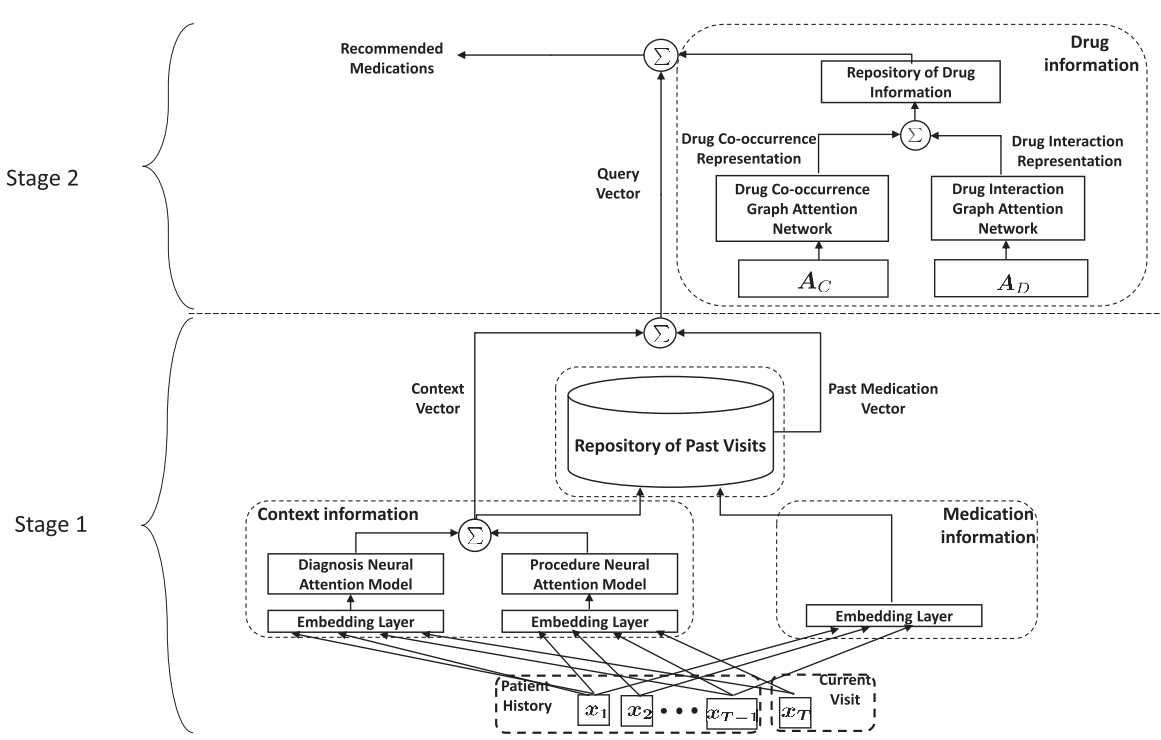
\includegraphics[width=8.5cm, height = 7.5cm]{PREMIER.png}
    \caption{PREMIER's two Stage Recommender System \cite{Bhoi2021 as}.}
    \label{one}
\end{figure}

Recurrent Neural Networks are a popular architectural choice for mimic-based RS
mainly because of their memory ability which is vital for training on user
visits \cite{Wang}. PREMIER \cite{Bhoi2021} is a two-stage attention-based
RS. Figure \ref{one} shows the architecture with information about each stage. In
the first stage, the system uses past diagnoses and procedures and embeds
this information into the RNN. In the second stage, they combine the
second dataset of drug interactions to ensure that each recommendation is
safe for the user. The system also justifies the recommendations by
splitting them into two parts; one for the diagnosis and one for the
procedures, and uses a weight feature to calculate the importance. As a
result, PREMIER outperforms state-of-the-art medication recommendation
systems while achieving the best tradeoff between accuracy and drug-drug
interaction.  

Finally, Wang et al. \cite{Wang} proposed a solution that uses Supervised Reinforcement
Learning with RNNs on the Mimic Dataset. They contain an off-policy
actor-critic architecture to discover unique optimal personalised
treatments and evaluated that their system can decrease the estimated
mortality in hospitals by up to 4.4\%.



\section{Proposed Idea}
    Health RS plays an essential role in food, diet, and physical activity
recommendation, and RS research is growing fast, especially in the e-commerce
sector \cite{Tran2021b}. However, the RNN prediction solutions
like Wang et al. \cite{Wang} and PREMIER \cite{Bhoi2021} only incorporate past diagnoses and past
procedures. Our proposed solution for this study is to use the vast amount of
data in EHR like MIMIC in the RS.  The following describes our proposed ways of
tackling the objectives.


\subsubsection{
    Tackling cold start issues for new patients
}

The more features the system contains, the more it can handle cold start issues
for new patients with little data. For example, if the system is trained on the
age, diagnoses and procedures and a new user only has the first two, the system
should be capable of recommending the right medicine. 

\subsubsection{
Finding the best Model
}
After splitting the dataset into a training set and a testing set, we would
like to find the best model that achieves the highest scores.

\subsubsection{
    Preventing adverse side effects from recommendations
}
We can aggregate the EHR dataset with a drug interactions dataset containing
information about a specific medication and its effects and conflicts with
other drugs. This combination ensures that any recommended medicine does not
cause harm or damaging side effects to any patients. 

\subsubsection{
    Selecting the best features from the dataset
}
Choosing the best features from the EHR dataset helps us build an efficient
model. Our goal is to determine which data hold value for increasing accurate
predictions.


\subsection{
The Dataset 
}
The MIMIC (Medical Information Mart for Intensive Care) is a publicly
available EHR dataset under the registration of the university of MIT
containing data from patients admitted to the critical care units of the Beth
Israel Deaconess Medical Center \cite{Johnson2016}.

There are four versions of this database, and after applying, we have been
given access to MIMIC III and MIMIC IV. The third version contains twenty-six
tables, over 40,000 patient records (excluding people under 16), and 53,423
visits between 2001 and 2012. Each patient is de-identified and anonymised and
contains medical intake, chart events, ICU date stays, demographics, doctor's
notes and more. On average, each patient has around 2.68 visits, and table \ref{age}
shows some statistics about the dataset, and figure \ref{statistics} shows the age
distribution of the patients. People over 90 are grouped. Each patient is
identified with a patient ID, used throughout the tables. Diagnosis, Procedures
are encoded using international standards such as ICD-9 and ATC classification .

\begin{figure}[h]
    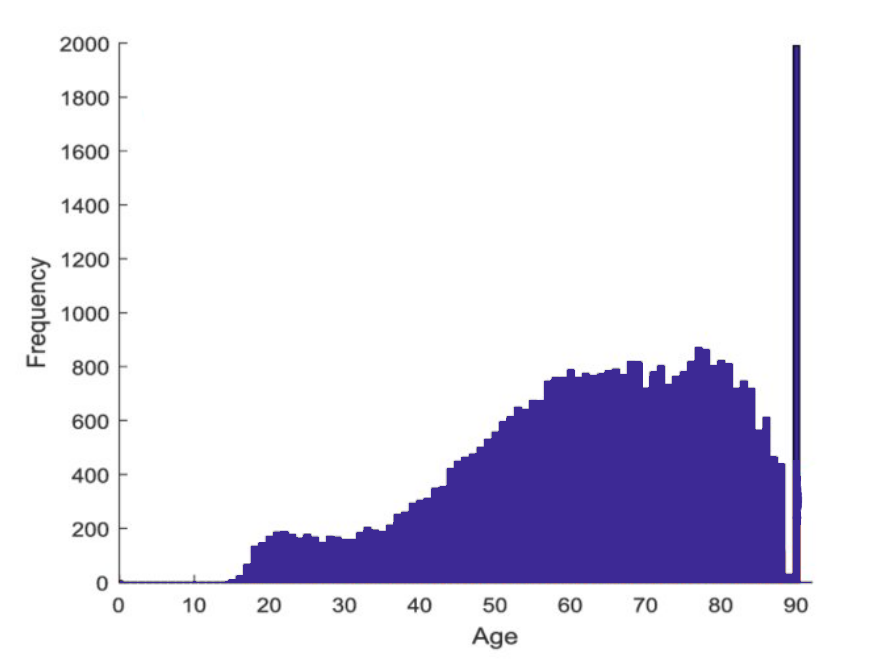
\includegraphics[width=8.5cm, height = 6cm]{ageDistribution.png}
    \caption{Age Distribution of MIMIC III}
    \label{age}
\end{figure}


\begin{table}[h]

    \caption{MIMIC III Statistics.}
    \label{statistics}
\begin{center}
\begin{tabular}{ | c | c | }
    \hline
 Number of patients     & 46520 \\ 
    \hline
 Number of Diagnoses    & 14567 \\  
    \hline
 Number of Procedures   & 3882  \\
    \hline
 Number of Medicine     & 4204  \\
    \hline
\end{tabular}
\end{center}

    \end{table}


\subsection{Testing and Evaluation}

There are three main things to test for evaluating the RS, performance,
accuracy scores and drug interactions tests. These three measures will
ensure that our system would recommend good medicine as fast as possible
whilst also ensuring the patient's safety. We will also compare our
system's safety with other RS using standard drug interactions metrics.

We will also split the dataset into training, testing, and validation sets
to calculate additional evaluation metrics such as the F1 score,
precision,Jaccard, Root-mean-square deviation, and Mean Absolute Errors. Doing so
will allow us to compare our system with existing systems that use the
MIMIC dataset. We could also package the system in an application and
present sample use cases to demonstrate our system. 




\section{Conclusion}

This proposal presents a medicine recommender system that could
personalise medicine prescriptions to a patient. The system will need
to generate fast, safe and accurate results for the end-user. The field of
RS is continuously growing. It would be beneficial to incorporate 
modern techniques such as Collaborative Filtering or Content-based Filtering
with a health dataset like the MIMIC III or MIMIC IV, to which we
already have access. This study contributes to both the field of
Recommender Systems and Precision Medicine.

\bibliographystyle{IEEEtran}
\bibliography{/home/liamattard/Documents/Masters/bibtex/AImasters}

\end{document}
